 \documentclass[11pt]{article}

\usepackage[english]{babel}
\usepackage[margin=1in]{geometry}

% Math/Greek packages
\usepackage{amssymb,amsmath,amsthm, mathtools} 
\usepackage{algorithm, algorithmic}
\usepackage{upgreek, siunitx}
\usepackage{setspace}

% Graphics/Presentation packages
\usepackage{multirow}
\usepackage{graphicx}
\usepackage{cancel}
\usepackage{tabulary, enumitem, array}
\usepackage{xparse,mleftright,tikz}
\usepackage{physics}

% Misc packages
\usepackage{fancyhdr}


\usepackage[export]{adjustbox}

\usepackage{esint}

\sisetup{locale=US,group-separator = {,}}
\usepackage[colorlinks=true, allcolors=blue]{hyperref}


\begin{document}

\title{PHSX 462: HW07}
\author{William Jardee}
\maketitle


\section*{Question 1}
We provided 
\[\dd{N} = \frac{V}{2\pi^2}\left(\frac{2m}{\hbar^2}\right)^{3/2}E^{1/2}\dd{E}\]
in class, so let's start with that.

\begin{align*}
E_{\text{total}} & = \int_0^N E\dd{N} \rightarrow \int_0^{E_F} E \left[\frac{V}{2\pi^2}\left(\frac{2m}{\hbar^2}\right)^{3/2}E^{1/2}\dd{E}\right]\\
& = \frac{V}{2\pi^2}\left(\frac{2m}{\hbar^2}\right)^{3/2}\int_0^{E_F}E^{3/2}\dd{E}\\
& = \frac{V}{2\pi^2}\left(\frac{2m}{\hbar^2}\right)^{3/2}\frac{2}{5}\left(\frac{\hbar^2}{2m}\left(\frac{3N\pi^2}{V}\right)^{2/3}\right)^{5/2}\\
& = \frac{\hbar^2}{10\pi^2m}\frac{(3\pi^2N)^{5/3}}{V^{-2/3}} \qquad \checkmark
\end{align*}

%--------------------------------------------------------------------------------
\newpage

\section*{Griffiths 5.21}
\begin{enumerate}[label=\alph*)]
\item We know that $\displaystyle{E_F = \frac{\hbar^2}{2m}\left(3\rho\pi^2\right)^{2/3}}$. The density, $\rho$, here is the density of electron; so, it will be
\[\rho = 8.96 \frac{\text{g}}{\text{cm}^3} \cdot \frac{1}{63.5}\frac{\text{mole}}{\text{g}} \approx 0.1411 \frac{\text{mole}}{\text{cm}^3} \approx \boxed{8.4974 \times 10^{28}\, \frac{\text{electrons}}{\text{m}^3}}\,.\] 
Using the value of $m = 0.511 \text{Mev}/\text{c}^2$ and $\hbar = 6.582 \times 10^{-16} \text{eV}\, \text{s}$ the calculation yields
\[\boxed{E_F \approx 7.842 \times 10^{-17} \, \text{eV}}\,.\]

\item We can assume that there is no potential energy, and these are non-relativistic particles, so 
\[E_F = \frac{1}{2}mv^2 \rightarrow v = \sqrt{\frac{2E}{m}} \approx 1.752 \times 10^{-11} \, c \approx \, \boxed{5.256 \times 10^{-3} \frac{\text{m}}{\text{s}}}\,.\]

\item This is as simple as evaluating 
\[T = \frac{E_F}{k_B} \approx \boxed{9.0998\times 10^{-13}\,\text{K}}\,.\]

\item Again, just ``plug and chug":
\[P = \frac{\left(3\pi^2\right)^{2/3}\hbar^2}{5m}\rho^{5/3} \approx \boxed{2.3988 \times 10^{29} \frac{\text{eV}}{\text{m}^3}}\,.\]
\end{enumerate}

%--------------------------------------------------------------------------------
\newpage

\section*{Griffiths 5.30}
We need to start by describing the wave function of our 2D well as
\[\psi_{n_x \, n_y} = \sqrt{\frac{4}{A}}\sin(k_x \, x)\sin(k_y \, y).\]
With a corresponding energy $\displaystyle{E_k = \frac{\hbar^2\abs{\vb{k}}^2}{2m}}$, where $\vb{k} = k_x\hat{x}+k_y\hat{y}$ is the wavenumber. Considering this as a problem in a 2D wavenumber space, opposed to a quantum number space, the area spanned by each wave number is
\[\frac{\pi}{l_x} \cdot \frac{\pi}{l_y} = \frac{\pi^2}{A},\]
where $l_x$ and $l_y$ are the length of the well in $x$ and $y$ directions, respectively. 

The total area covered by the ground state, in the wavenumber space, is $\displaystyle{A_F = \frac{1}{4}\left(\pi k_F\right)^2}$, where $k_F$ is the largest wavenumber reached, relating to the Fermi energy, etc. The total number of electron ``squares" needed will be 
\[N_{\text{electrons}} = 2 \cdot N_{\text{squares}} = 2 \, \frac{A_F}{(\text{area per cube})} = 2 \, \frac{\frac{1}{4}\left(\pi k_F\right)^2}{\frac{\pi^2}{A}} = \frac{A k^2_F}{2\pi}.\]
Solving this for the wavenumber of the Fermi energy gives
\[k_F = \sqrt{\frac{2\pi N}{A}} = \sqrt{2\pi \sigma},\]
where $\sigma$ is the density of states. The Fermi energy is then
\[E_F = \frac{\hbar^2}{2m}k_F^2 = \boxed{\frac{\hbar^2 \pi}{m}\sigma}\]

%--------------------------------------------------------------------------------
\newpage

\section*{Griffiths 5.35}
\begin{enumerate}[label=\alph*)]
\item Starting with the total energy of the system
\[E_{\text{total}} = \frac{\hbar^2 \left(3\pi^2 N\right)^{5/3}}{10\pi^2 m}V^{-2/3}\]
and substituting what we know, overloading some of the terms, 
\[E_{\text{total}} = \frac{\hbar^2 \left(3\pi^2 Nd\right)^{5/3}}{10\pi^2 m}\left(\frac{4}{3}\pi r^3\right)^{-2/3}.\]
Simplifying this dramatically yields
\[\boxed{E_{\text{total}} = \frac{\hbar^2}{10m}\left(\frac{3\pi}{4}\right)^{2/3} \frac{(3Nd)^{5/3}}{r^2}} \, .\]

\item Grabbing this equation from the all-knowing Google
\[W = - \frac{3}{5}\frac{G\left(M^\prime\right)^2}{R}.\]
This is the work it takes to create a dense sphere of radius $R$ that has mass $M$. For our problem this looks like 
\[\boxed{U = -\frac{3}{5}\frac{G(NM)^2}{R}}\,.\]

\item The equation for the total energy is
\[E(r) = \frac{\hbar^2}{10m}\left(\frac{3\pi}{4}\right)^{2/3} \frac{(3Nd)^{5/3}}{r^2} - \frac{3}{5}\frac{G(NM)^2}{r}.\]
Maximizing this, with respect to $r$ gives
\[ \dv{E}{r}  = -\frac{\hbar}{5m}\left(\frac{3\pi}{4}\right)^{2/3}\frac{(3Nd)^{5/3}}{r^3} + \frac{3}{5}\frac{G(NM)^2}{r^2} = 0, \]
\[r  = \frac{\frac{\hbar^2}{m}\left(\frac{3\pi}{4}\right)^{2/3}(3Nd)^{5/3}}{3G(NM)^2} = \boxed{ \left(\frac{9\pi}{4}\right)^{2/3} \frac{\hbar^2 d^{5/3}}{GmM^2N^{1/3}}}\, .\]

Plugging in $m = 0.511 \text{MeV}/c^2$, $M = 939 \text{MeV}/c^2$, $d = 1/2$, $G = 6.674 \times 10^{-11} \text{N} \, \text{m}^2 / \text{kg}^2$ give $\displaystyle{\boxed{R \approx 7.6 \times 10^{25} \, N^{-1/3} \, \text{m}}}\, .$

\item Using the mass of the sun, $M_\text{Sun} = 1.989\times 10^{30} \text{kg}$, and the fact that $N = M_\text{Sun}/M$, 
\[\boxed{R \approx 7.16 \times 10^6 \text{m}}\, .\]

\item The Fermi energy is 
\[E_F = \frac{\hbar^2}{2m}\left(3 \rho \pi^2\right)^{2/3} = \frac{\hbar^2}{2m}\left(3 \frac{N}{\frac{4}{3}\pi R^3}\pi^2\right)^{2/3}\]
where $R$ and $N$ are the same as the last part. Plugging in values we get
\[\boxed{E_F \approx 1.94\times 10^5 \text{eV}} \, .\]

\end{enumerate}

%--------------------------------------------------------------------------------
\newpage

\section*{Griffiths 5.25}
We want the lowest energy, so that will be the solution to 
\[\cos(qa) = cos(ka)+ \frac{m\alpha}{\hbar k}\sin(ka)\]
when the $n$ embedded in $q$ is zero. Since $\displaystyle{q = \frac{2\pi n}{Na} \rightarrow 0}$, and we are given that $\beta$ (the jazz in front of the sin) is 10, the problem is really
\[1 = \cos(z) + 10 \frac{\sin(z)}{z}\]
where $z = ka$. Using digital software, $z \approx 2.628$. 

Given that $\displaystyle{k = \frac{\sqrt{2mE}}{\hbar}}$, $\displaystyle{\beta = \frac{m\alpha a}{\hbar^2}}$, $\beta = 10$, and $\alpha / a = 1 \text{ eV}$, $E$ can be solved for. Rearanging the $\beta$ equation gives that 
\[a^2 = a \frac{\beta \hbar^2}{m\alpha} = \frac{\beta \hbar^2}{m}\left(\frac{\alpha}{a}\right)^{-1} = \frac{10 \hbar^2}{m} \text{ eV} \, .\]
Solving for $E$ from the $k$ equation, and substituting what $a^2$ is gives
\begin{align*}
E & = \frac{z^2\hbar^2}{a^2}\frac{1}{2m} = \frac{z^2h\hbar^2m}{10\hbar^22m} = \frac{(2.628)^2}{20}\text{eV}\\
& \approx \boxed{0.345 \text{ eV}}
\end{align*}

%--------------------------------------------------------------------------------
\newpage

\section*{Griffiths 5.26}
We get back to the same differential equation as in the book; 
\[\dv[2]{\psi}{x} = -\frac{2mE}{\hbar^2}\psi \, .\]
For the case when $E>0$, the solution follows exactly as in the book. If we assume that $E<0$, then the general solution is instead 
\[\psi(x) = A\sinh(kx) + B\cosh(kx) \, . \]
Using Bloch's theorem, we know that if we move left a cell the solution can also be
\[\psi(x) = e^{-iqa}\left[A\sinh(kx) + B\cosh(kx)\right] \, . \]

At the point $x=0$, these solution must be equivalent; that is
\[B = e^{-iqa}\left[A\sinh(ka) + B\cosh(ka)\right] \, .\]
Solving for $A$ gives
\[A = \left[Be^{iqa} - B\cosh(ka)\right]\left(\sinh(ka)\right)^{-1} \, .\]
Following equation 2.128 in the book $\displaystyle{\left(\Delta\dv{\psi}{x} = \frac{2m\alpha}{\hbar^2}\psi(0)\right)}$, we get
\[kA - e^{-iqa}k\left[A\cosh(ka) + B\sinh(ka)\right] = \frac{2m\alpha}{\hbar^2}B \, .\]

Substituting in the $A$ that we got earlier, and doing some simplification gives
\[k\left[Be^{iqa} - B\cosh(ka)\right]-e^{-iqa}\left[\left(Be^{iqa} - B\cosh(ka)\right)\cosh(ka) + B \sinh[2](ka)\right] = \frac{2m\alpha}{\hbar^2}B\sinh(ka) \, ,\]
\[k\left[e^{iqa} - 2\cosh(ka) + e^{-iqa}\right] = \frac{2m\alpha}{\hbar^2}\sinh(ka) \, ,\]
\[\boxed{\cos(qa) = \frac{m\alpha}{\hbar^2 k} \sinh(ka) + \cosh(ka)} \, .\]

The negative solution is monotonically decreasing, so there is only one band that is added here. Just like with the positive bands, there will be a total of $N$ intersections, and thus $N$ states.

\vfill
\textit{See next page for graph.}

\begin{figure}[!ht]
\centering
	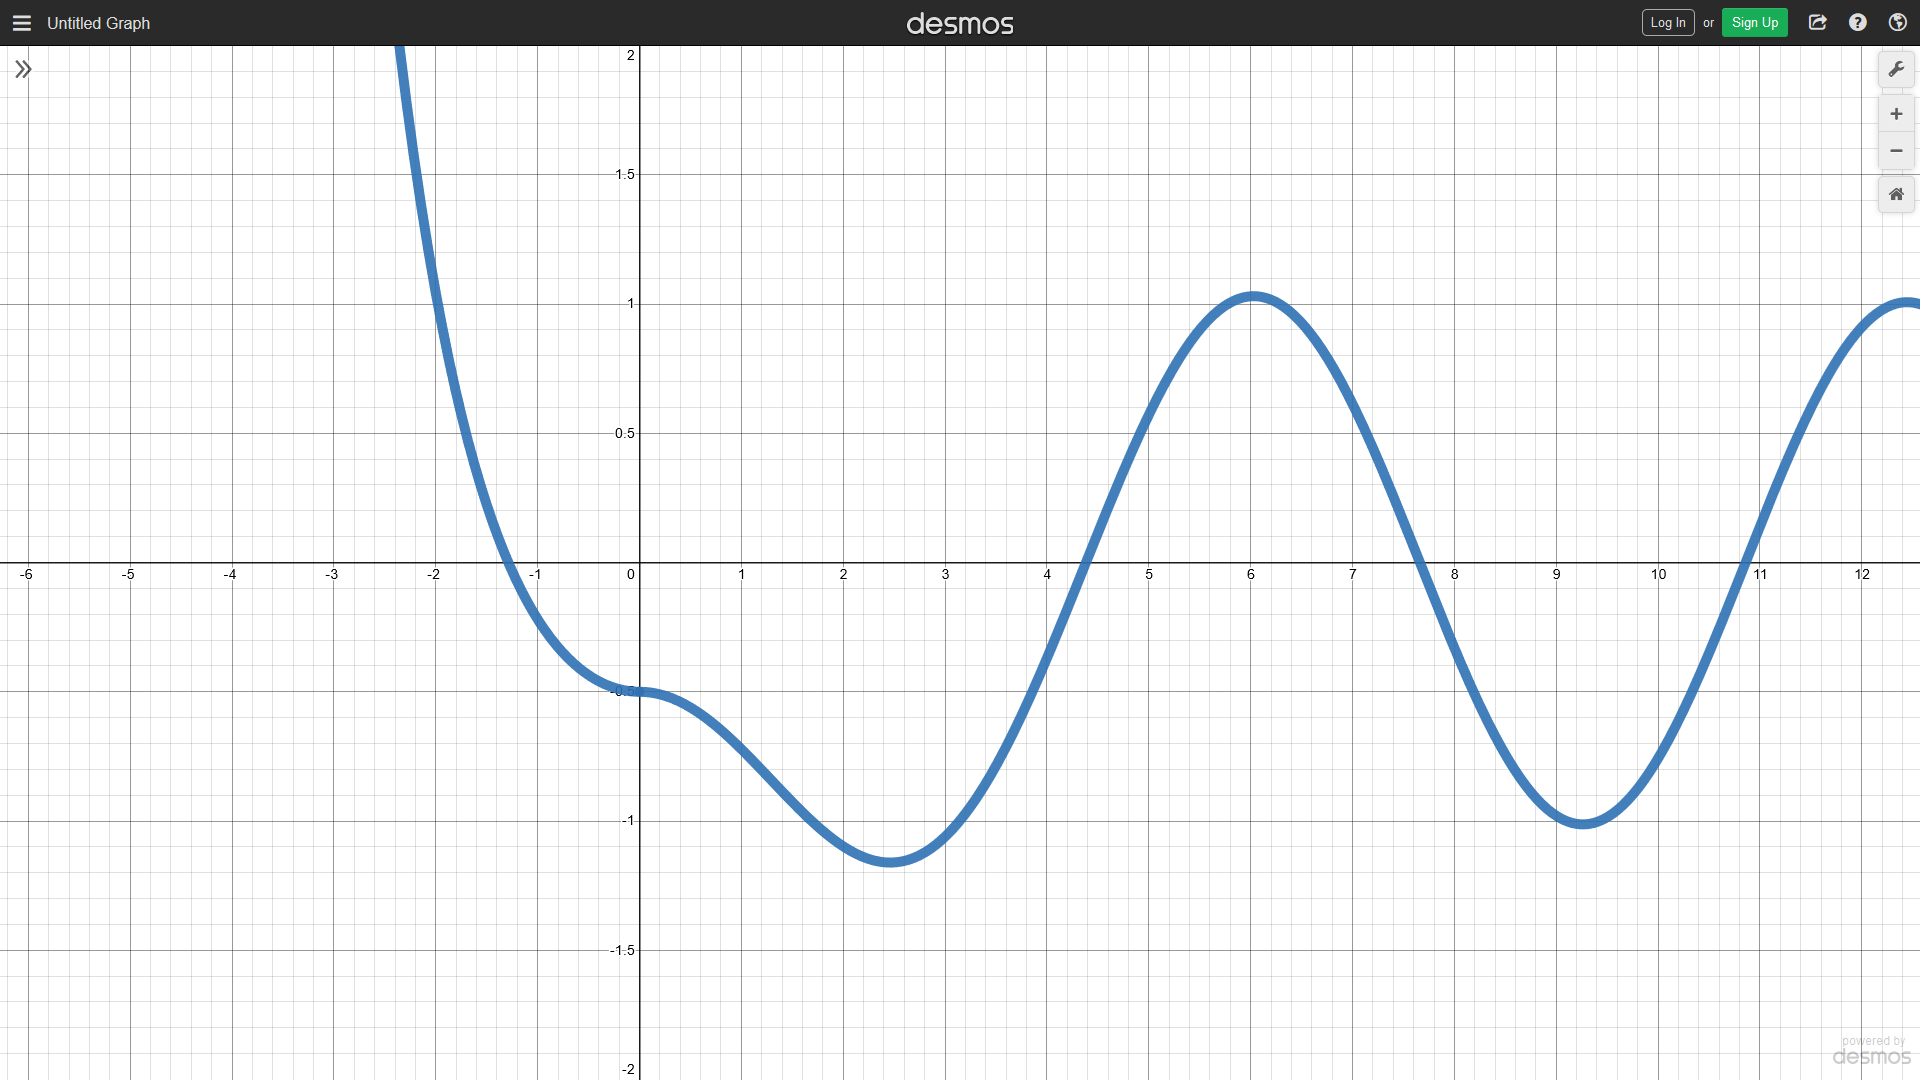
\includegraphics[width=0.9\linewidth]{phsx462_hw07_01.PNG}
	\caption{The plot for the dirac delta wells. The x-axis, which represents $z$, is plotted from -$2\pi$ to $4\pi$ with negative $z$ being the negative energy solution and positive the solution given in the book. The y-axis runs from -2 to 2.}
	\label{fig:6.1}
\end{figure}

\end{document}
